\subsection{Overview}
As stated above, each subsystem has to accomplish its own goals. In particular, we can consider AutomatedSOS and Track4Run as simple  applications for smart-devices, while Data4Help as a service provider that should implement a more complex, scalability-oriented architecture.

The figure below represents the physical architecture of the system to-be.

\FloatBarrier
\begin{figure}[!h]
	\centering
	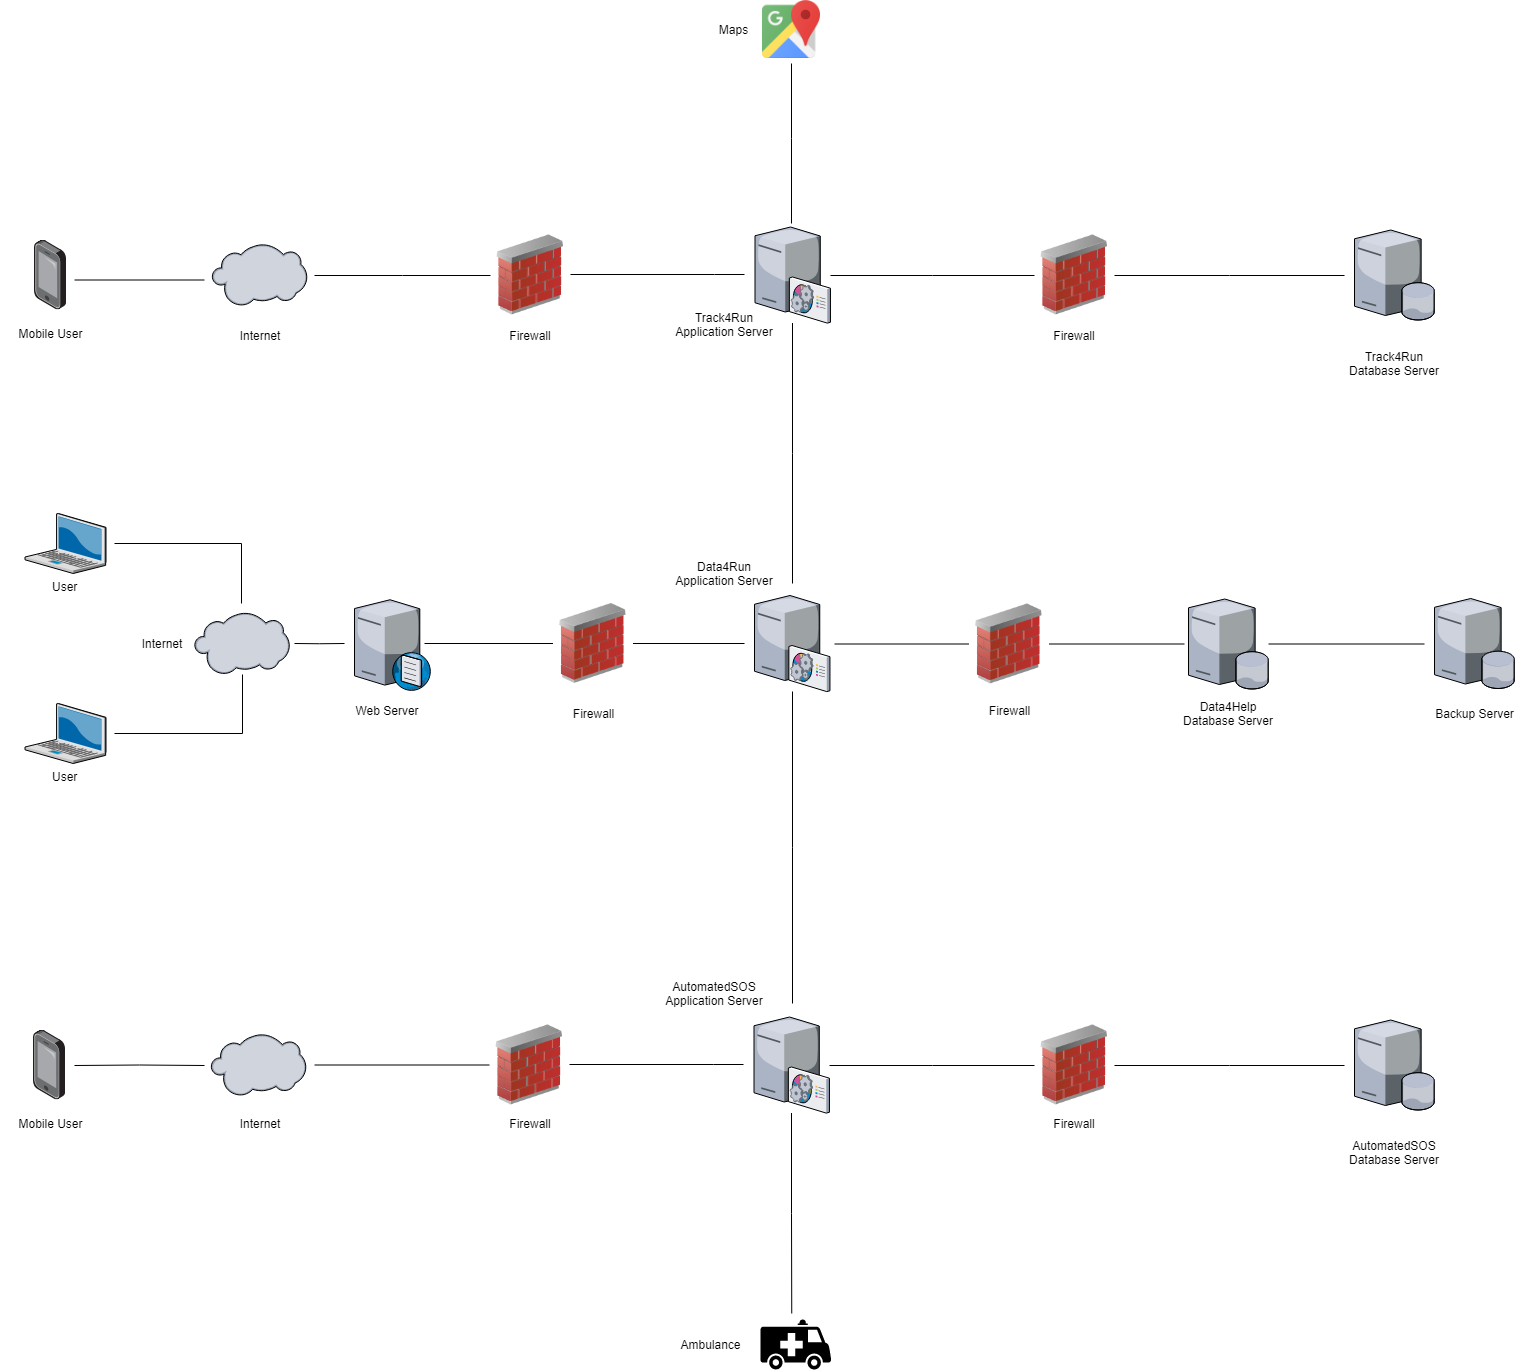
\includegraphics[width=0.9\columnwidth]{physicalArchitectureDiagram.png}
	\caption{General Architecture}
\end{figure}
\FloatBarrier

As shown in the figure, Data4Help services can be accessed through different channels. In particular, we provide a web interface for the end users and an API for data sources and third party applications.

Since the data sources will continuously provide the system with real-time user data, we expect that this flow of information will soon grow into a huge number of requests. For this reason, this subsystem has to be designed to guarantee high scalability and to ensure a high availability level even in extreme conditions.
In particular, a microservice-based architecture coupled with message queues and scalable databases should be adopted, as we will describe in the following sections. Finally, an API Gateway is used to access all Data4Help interfaces, in order to easily manage the authentication phase and load balancing from the very first moment of any request.

On the other hand, AutomatedSOS and Track4Run are designed as three-tier applications with a thick client (i.e. smart-phones and smart-watch applications), a lightweight back-end server and a storage module. 
In the design of these two subsystems we applied the separation of concerns principle for different reasons:

\begin{enumerate}
    \item Modularity: AutomatedSOS and Track4Run business logic are separated from Data4Help business logic.
    \item Back-end performances: we ensure a fast and reliable service leaving the presentation part to the mobile application.
    \item System maintainability: multi-layered architecture and the achieved modularity helps long term maintainability.
    \item Mobile devices performances: considering that CPU usage and power consumption are significant issues, we lighten their workload.
\end{enumerate}

\subsection{High Level Architecture}
From the component point of view, each subsystem can be divided into \textit{back-end} components, which are responsible of carrying out the business logic of the subsystem, and \textit{front-end} components, which provide a presentation layer to the end users and SDKs to the external developers who want to access the system's services. 
Finally, we rely on some external components to provide some of the services offered by the system.

In the following diagram, the main components and interfaces are highlighted, to give a general idea of the system design.
Components and modules represent a set of services grouped together, and the internal interactions between modules are not shown for sake of simplicity. This description will be done in the following sections.

\FloatBarrier
\begin{figure}[!h]
	\centering
	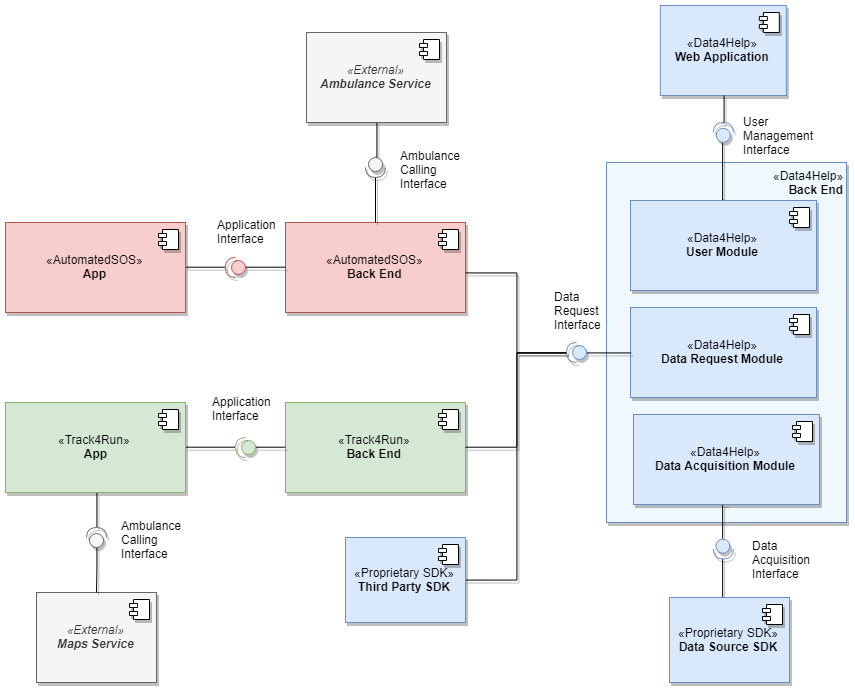
\includegraphics[width=\columnwidth]{ComponentDiagrams-Total.png}
	\caption{High Level Components}
\end{figure}
\FloatBarrier

As can be seen, the Data4Help back-end consists of four major modules:

\begin{itemize}
	\item \textbf{User Management}: provides an interface for managing the user account and configure his data sources. This interface is used by a \textit{Web Application} that can be accessed via web browser.
	\item \textbf{Data Acquisition}: provides the interface for collecting data from data sources. A proprietary \textit{Data Source SDK} is given to the external developers to integrate the use of this interface into their software and send data from external devices to Data4Help.
	\item \textbf{Data Request}: enables third parties to make requests on the data received by the subsystem. This interface is used by \textit{Track4Run} and \textit{AutomatedSOS} back-ends, but it can also be accessed by any other third party via the dedicated \textit{Third Party SDK} given to their developers.
	\item \textbf{Authentication}: enables the system to recognize and authenticate incoming requests and associate them to a specific user, third party or data source.
\end{itemize}

The other two back-ends are mainly responsible of exploiting Data4Help's services and offer an interface to the mobile application. In particular:

\begin{itemize}
	\item \textbf{AutomatedSOS App Interface}: provides the functions to log in a user, modify its threshold and monitor its health status.
	\item \textbf{Track4Run App Interface}: provides the functions to log in a user, create and edit a run, search for scheduled events, join them and watch runners during a competition.
\end{itemize}

Finally there are the external services: for AutomatedSOS, an external Ambulance Calling Interface is needed by the back-end to fulfill its goals; Track4Run instead needs a Maps Service such as \textit{Google Maps} that should be accessed directly from the application to minimize latency and bandwidth occupation in the communication between client and server.

Another definition of the services offered by the system can be found in the figure below, which highlights the dependencies between the Data4Help system and its actors providing a list of the services used internally and externally by the system.

\FloatBarrier
\begin{figure}[!h]
	\centering
	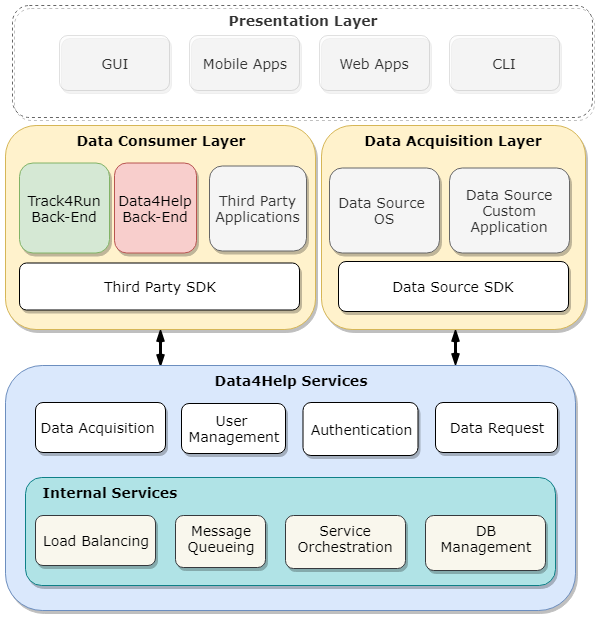
\includegraphics[width=0.8\columnwidth]{ComponentDiagrams-Layers.png}
	\caption{System Layers Architecture}
\end{figure}
\FloatBarrier

The whole system's internal and external services can be divided into five layers:

\begin{itemize}
	\item \textbf{Data4Help Internal Services Layer}: these components are used internally by Data4Help to provide highly available services. They mainly deal with microservices management and will not be discussed in detail, since there are many available options on the market such as Docker and Kubernetes for container management, MongoDB for data management, RabbitMQ for message queueing, Prometheus for monitoring etc...
	\item \textbf{Data4Help External Services Layer}: this layer provides the four main functionalities of Data4Help, which have been discussed previously.
	\item \textbf{Data Acquisition Layer}: this layer is built upon Data4Help Services. It contains the SDK on which external data sources can rely on to send collected data to Data4Help.
	\item \textbf{Data Consumer Layer}: also this layer is built upon Data4Help Services and contains the SDK to send API requests used by third parties as well as AutomatedSOS and Track4Run back-ends, which can be seen as \textit{consumers} of the Data4Help services.
	\item \textbf{Presentation Layer}: built upon the previous layers. It is the mobile application of AutomatedSOS and Track4Run which provides a GUI to the end user.
\end{itemize}


\subsection{Component View}

\subsubsection{Data4Help}
Here is a detailed view of the components of the Data4Help subsystem: each service must be considered as independently deployed and can be replicated in many instances, following the typical microservice cluster architecture. 

\FloatBarrier
\begin{figure}[!h]
	\centering
	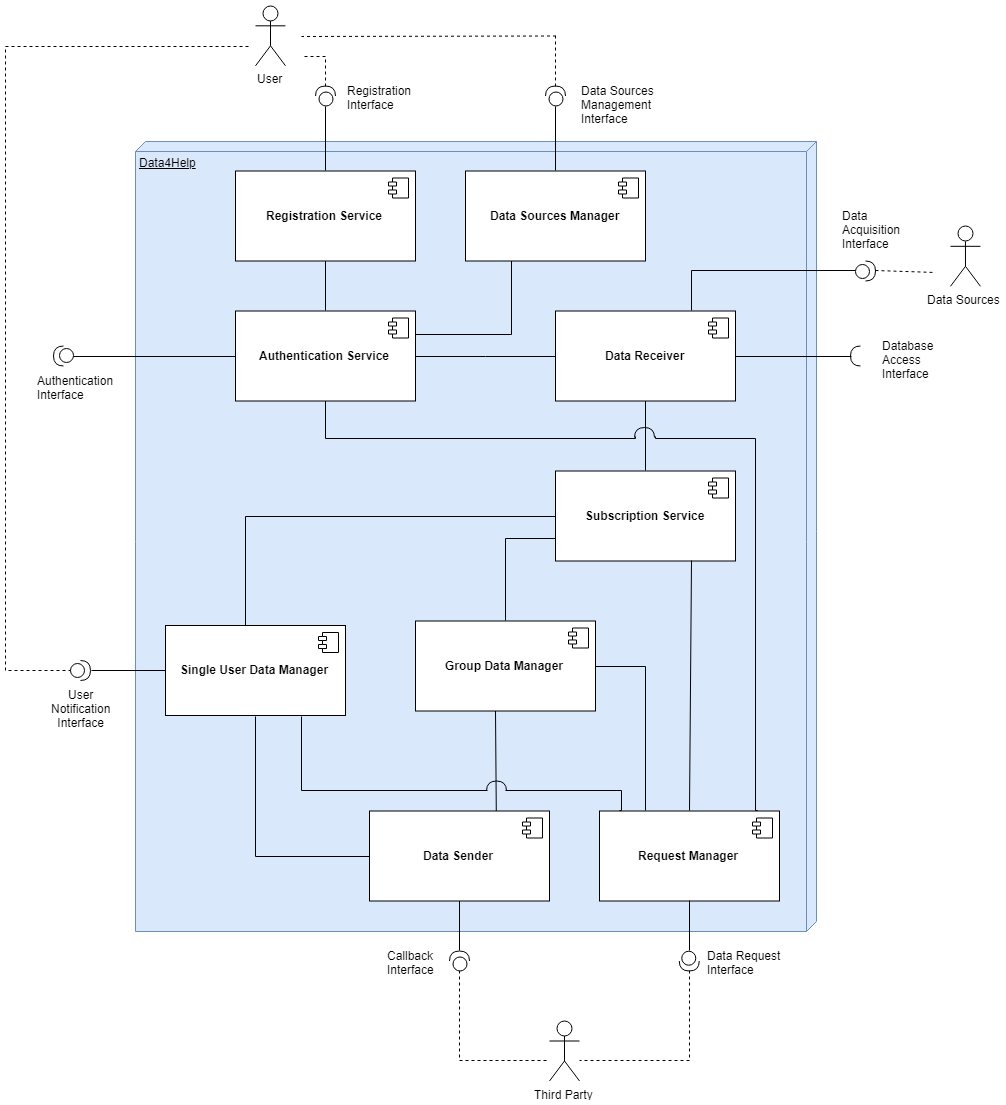
\includegraphics[width=\columnwidth]{ComponentDiagrams-Data4Help.png}
	\caption{Data4Help Components}
\end{figure}
\FloatBarrier

The components of this subsystem are:

\begin{itemize}
	\item \textbf{API Gateway}: This is the single entry point through which all other services can be accessed. For more information see \textit{API Gateway Pattern} in \textit{Section 2.7}. In this diagram, other components are also represented in the API Gateway:
	
	\begin{itemize}
		\item \textit{Load Balancer:} realizes the balancing between different instances of the same services, deciding where to redirect each request.
		\item \textit{Service Registry:} keeps track of all the deployed services instances.
		\item \textit{Service Orchestrator:} responsible of managing the deployment of new services and the failure of existing ones.
		\item \textit{Message Broker:} enables messaging between services.
		\item \textit{Performance Monitor:} continuously tracks end-to-end delay of our services and notifies the need for more resources. This component is needed to achieve high responsiveness of the system, in particular this is required to meet AutomatedSOS 5 seconds time constraint. 
	\end{itemize}
	
	Please notice that, for the sake of simplicity, the interaction between these components and the rest of the system is not represented here. As already mentioned, all these services are part of the internal services layer and are considered to be something already existing during the development of this subsystem.
	\item \textbf{Authentication Service:} in charge of producing tokens when new users register and verifying the incoming ones when requests are made to the API Gateway.
	\item \textbf{User Management Service:} provides an interface for the web application. The main functions are account management (password changing, name setting etc.) and data source management (i.e. selection of a data source for each tracked parameter).
	\item \textbf{Receiver:} responsible of managing a new incoming data source packet, verifying the user preferences for that data source and eventually saving the packet in the User Data DB. It is also responsible of notifying the subscription service with the ID of the received parameter, so that the interested third parties can be notified of the new data.
	\item \textbf{Request Manager:} responsible of receiving and parsing the data requests coming from third parties.
	In case of one-shot requests, a user notification service will be called to ask user's permission, and then the sender service will be invoked to send the actual response.
	If the request is instead a subscription request, this will be saved in the Requests DB after user's approval.
	Group requests don't need user approval, but they need to be filtered through the anonymization service.
	\item \textbf{User Notification:} provides a way to notify the user through different communication channels (e.g. e-mail, SMS, in-app notifications etc.) and receive his response.
	\item \textbf{Sender:} in charge of consuming the sender queue, build the request for each response and send it to the corresponding callback interface.
	\item \textbf{Subscription Service:} in charge of consuming the notifications received by the receiver service(s) and control if the new data fits into a single user or group data subscription. In this case, the corresponding response will be queued in the sender queue.
	\item \textbf{Anonymization Service:} simply tells if a given group request can be properly anonymized. It should be accessed using a synchronous protocol.
\end{itemize}

\subsubsection{AutomatedSOS}
AutomatedSOS follows the typical client-server architecture: in the back-end we have all the business logic of the application, while the presentation is carried out by the Client Application.

\FloatBarrier
\begin{figure}[!h]
	\centering
	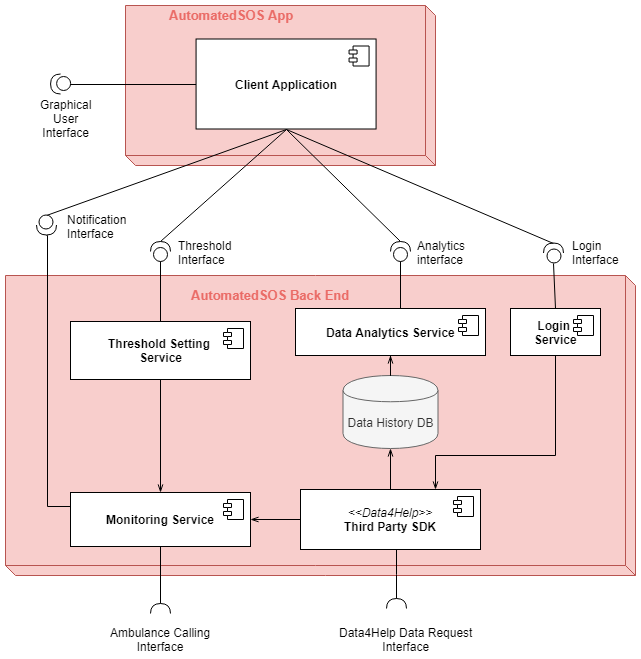
\includegraphics[width=\columnwidth]{ComponentDiagrams-AutoSOS.png}
	\caption{AutomatedSOS Components}
\end{figure}
\FloatBarrier

\begin{itemize}
	\item \textbf{Client Application:} application on user's device responsible of providing a graphical interface to the user and interacting with the back-end  services of AutomatedSOS.
	\item \textbf{Threshold Setting Service:} gives to the user the possibility to change the default threshold values of his tracked parameters and save them in the Threshold DB. 
	\item \textbf{Data Analytics Service:} allows the user to check the aggregated statistics about the data collected in a given time-lapse with a given granularity. 
	\item \textbf{Login Service:} responsible of authenticating the user with his Data4Help credentials using the Third Party SDK component. It also has to subscribe to the user's new data.
	\item \textbf{Monitoring Service:} receives the data coming from Data4Help through the SDK and, whenever a threshold is exceeded, interacts with the external Ambulance Calling Interface, communicating the location of the user in danger. The service gives priority to the data coming from users that are near to their thresholds using a sorted queue.
	\item \textbf{Third Party SDK:} communicates with Data4Help using his Authentication and Data Request interfaces.
\end{itemize}

\subsubsection{Track4Run}
Track4Run also follows the typical client-server architecture: in this case, the Client Application interacts not only with the back-end but also with an external Maps Interface.

\FloatBarrier
\begin{figure}[!h]
	\centering
	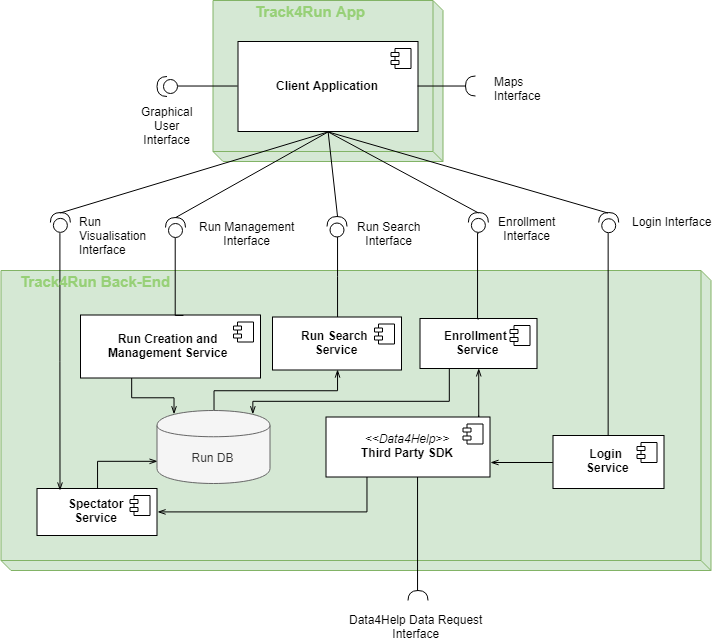
\includegraphics[width=\columnwidth]{ComponentDiagrams-Track4Run.png}
	\caption{Track4Run Components}
\end{figure}
\FloatBarrier

\begin{itemize}
	\item \textbf{Client Application:} application that runs on user's device responsible of providing a graphical interface to the user and interacting with the back-end services of Track4Run. It also interacts with an external Maps Interface in order to retrieve the maps that will be used by the application.
	\item \textbf{Run Creation and Management Service:} gives the user the possibility to create, edit, delete and extend ownership of a run event by interacting with the Run DB.
	\item \textbf{Run Search Service:} gives the user the possibility to browse all the created run events stored in the Run DB.
	\item \textbf{Spectator Service:} responsible of retrieving runners position during the run and then forwarding it to the Client Application which in turn will display the positions of the runners on a map.
	\item \textbf{Enrollment Service:} allows the user to enroll in a created scheduled run event. In this way he will be added to the list of participants.
	\item \textbf{Third Party SDK:} communicates with Data4Help using his Authentication and Data Request interfaces.
	\item \textbf{Login Service:} responsible of authenticating the user with his Data4Help credentials using the Third Party SDK component. It also has to subscribe to the user's new data.
\end{itemize}

\subsubsection{Entity-Relationship Diagram}
The following diagram provides a graphical representation of the data entities of the system. Different colours represent the three different subsystems.

\FloatBarrier
\begin{figure}[!h]
	\centering
	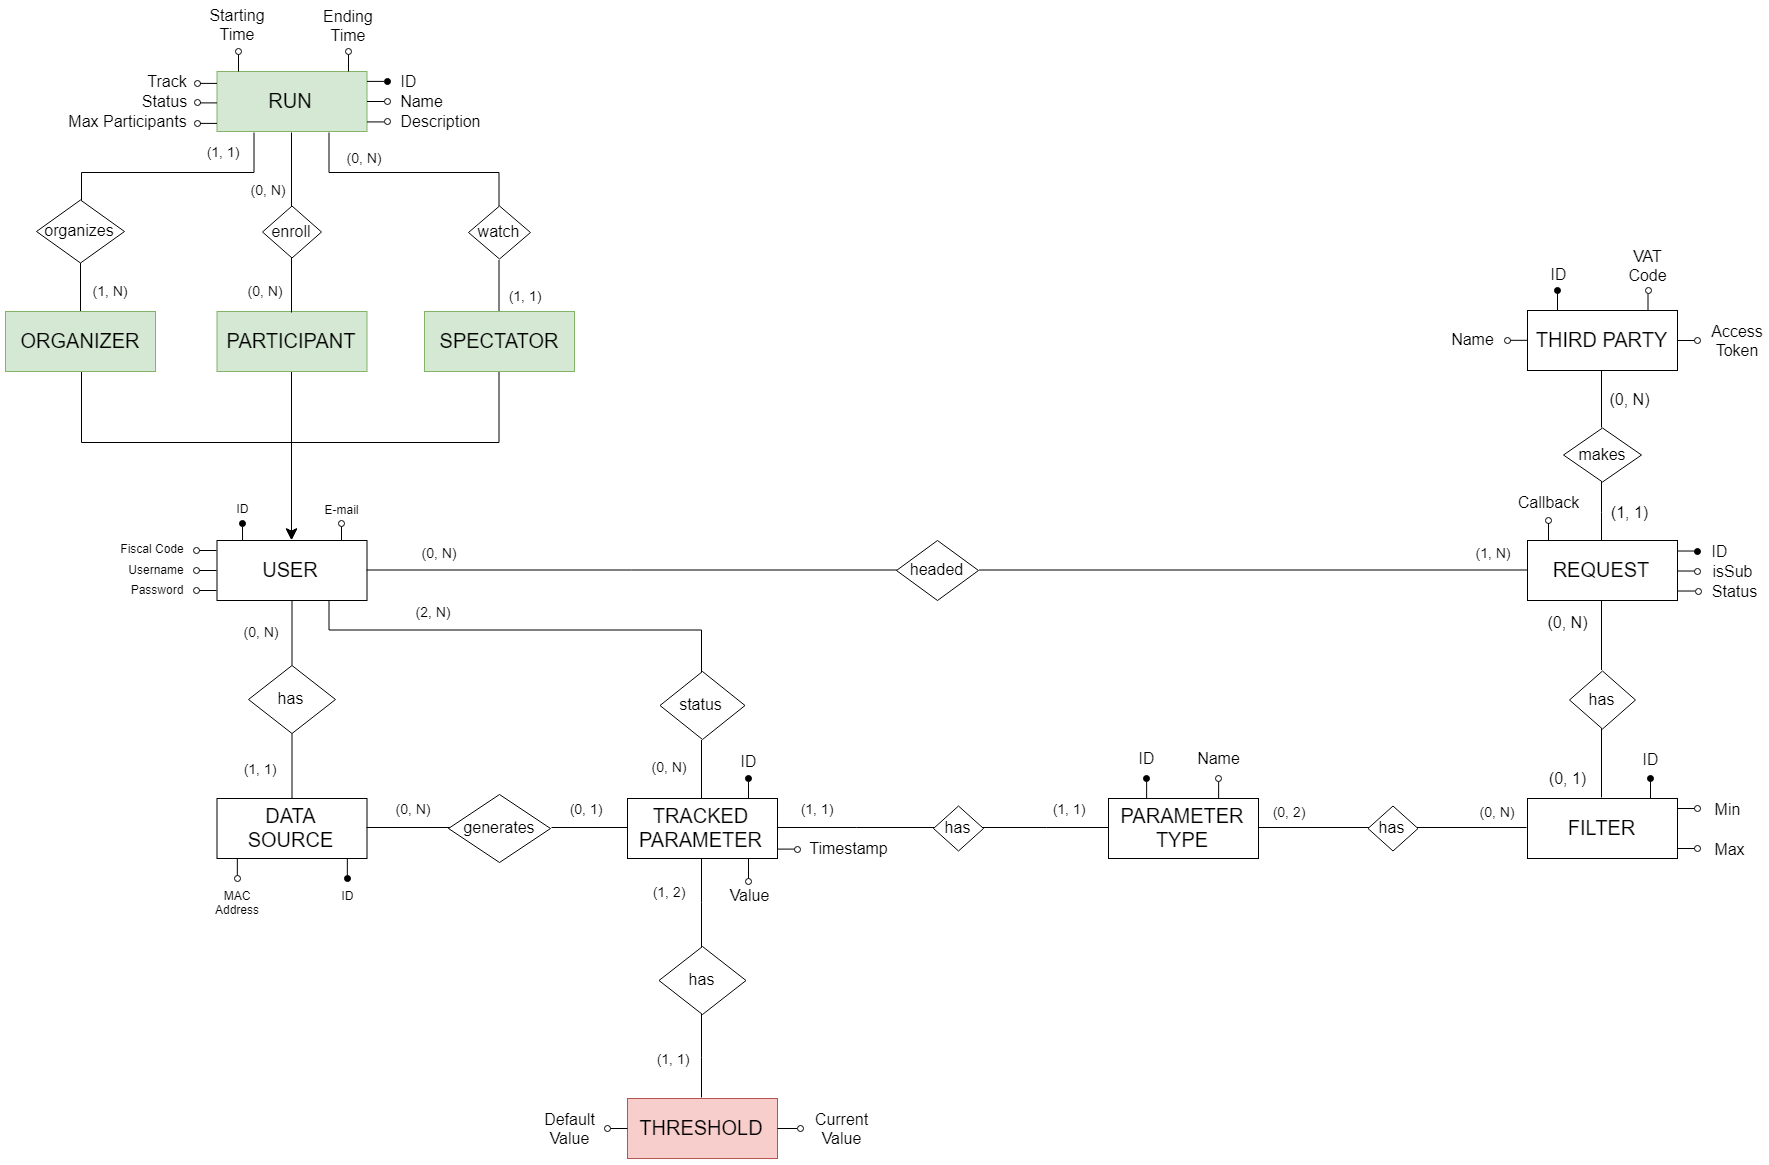
\includegraphics[width=\columnwidth]{ER.png}
	\caption{Entity-Relationship Diagram}
\end{figure}
\FloatBarrier

\subsection{Deployment View}
The deployment of the three subsystems reflects the architecture described in the previous sections. AutomatedSOS and Track4Run follow the client-server pattern, with a lightweight back-end (e.g. Servlet) and a DB server (SQL or NoSQL).

\FloatBarrier
\begin{figure}[!h]
	\centering
	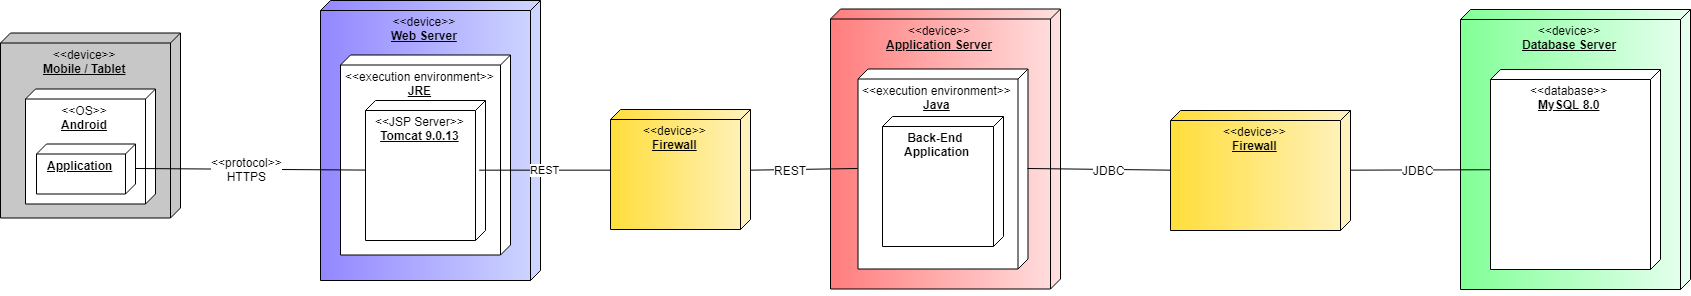
\includegraphics[width=\linewidth]{AppDepl.png}
	\caption{AutomatedSOS and Track4Run Deployment Diagram}
\end{figure}
\FloatBarrier

On the other hand Data4Help follows the microservices architecture pattern. In particular, the API Gateway and Server-Side Discovery patterns are applied: an \textit{API Gateway}, deployed on a dedicated machine, will filter all the incoming requests and forward them to the single services. To know where these services are located, a \textit{Service Registry} has to be deployed at a known address. Each back-end service is instead deployed in a separated \textit{container}, located in a physical or virtual machine, so that 
a new instance of a service can be deployed in a new container when needed. On the side of this microservice cluster, entities such as a Container Orchestrator, Load Balancer, Performance Monitor and a Message Broker are needed to properly manage the cluster. These have to be deployed in containers inside dedicated and reliable machines that are part of the internal network, to achieve scalability.

\FloatBarrier
\begin{figure}[!h]
	\centering
	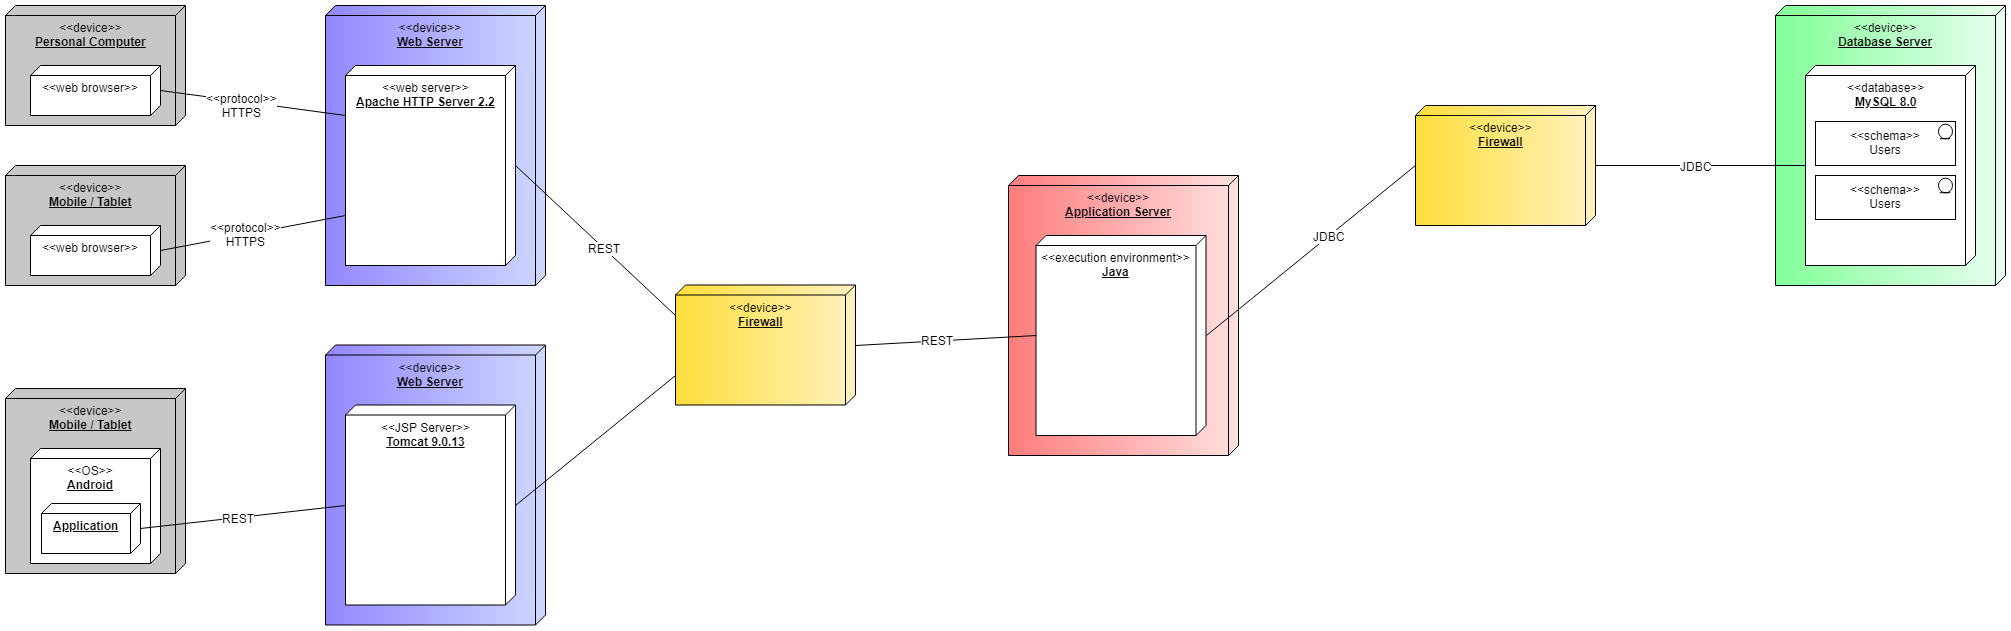
\includegraphics[width=\linewidth]{deploymentDiagram.png}
	\caption{Data4Help Deployment Diagram}
\end{figure}
\FloatBarrier

\subsection{Runtime View}
Many sequence diagrams have already been added in the RASD to show the interaction between the system and the users. Here some other internal details are provided for the four main functions of the Data4Help subsystem.

\subsubsection{Authentication}
Data4Help's authentication flow is taken from the classic token authentication pattern. Any \textit{Service Consumer} (i.e. end-users, third parties and data sources) can access the internal services if and only if they provide an access token previously generated by the system, during a login or registration phase.

\FloatBarrier
\begin{figure}[!h]
	\centering
	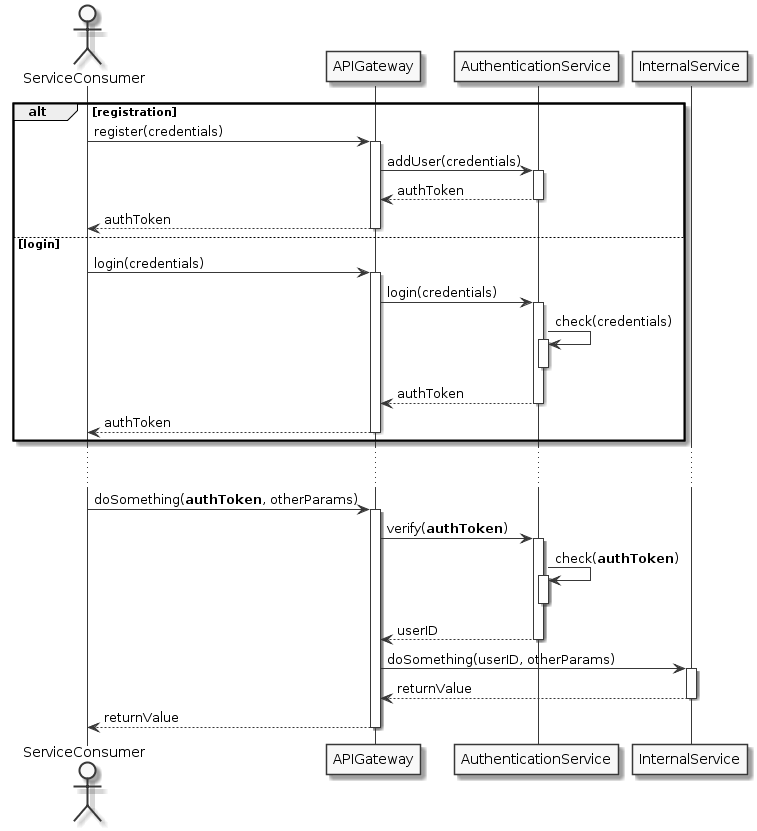
\includegraphics[width=\columnwidth]{auth_seq.png}
	\caption{Authentication Sequence Diagram}
\end{figure}
\FloatBarrier

\subsubsection{Data Acquisition}
Each time a new data is sent to the system, a Receiver must process that request and save the corresponding data on the User Data DB. Thereafter, an asynchronous notification will be sent to the Subscription Service to signal that a new data is ready to be sent.
When the Subscription Service is ready, it starts handling the notification: first it will check if some third party is subscribed to that specific user's data. Then, it will check if the new data is part of a data group and send the whole group's data to the subscribed third party if they can be properly anonymized.

\FloatBarrier
\begin{figure}[!h]
	\centering
	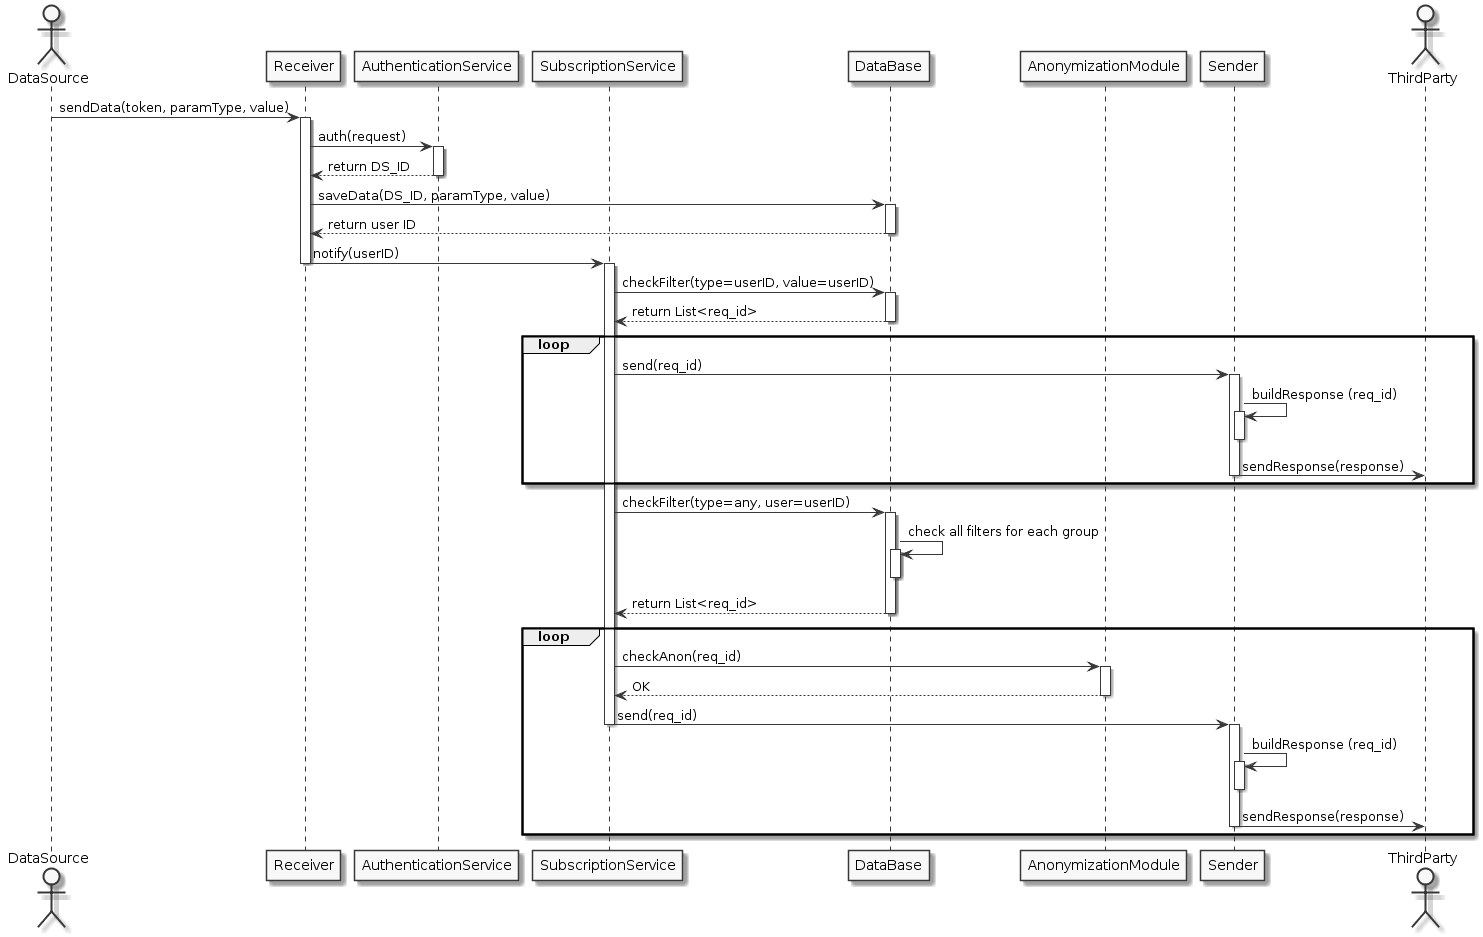
\includegraphics[width=\columnwidth]{newdata_seq.png}
	\caption{Data Acquisition Sequence Diagram}
\end{figure}
\FloatBarrier

\subsubsection{Single User Data Request}
In case a third party performs a single user data request, this request is marked as \textit{pending} until the target user approves it. This is true both for one-shot requests and subscription requests.

\FloatBarrier
\begin{figure}[!h]
	\centering
	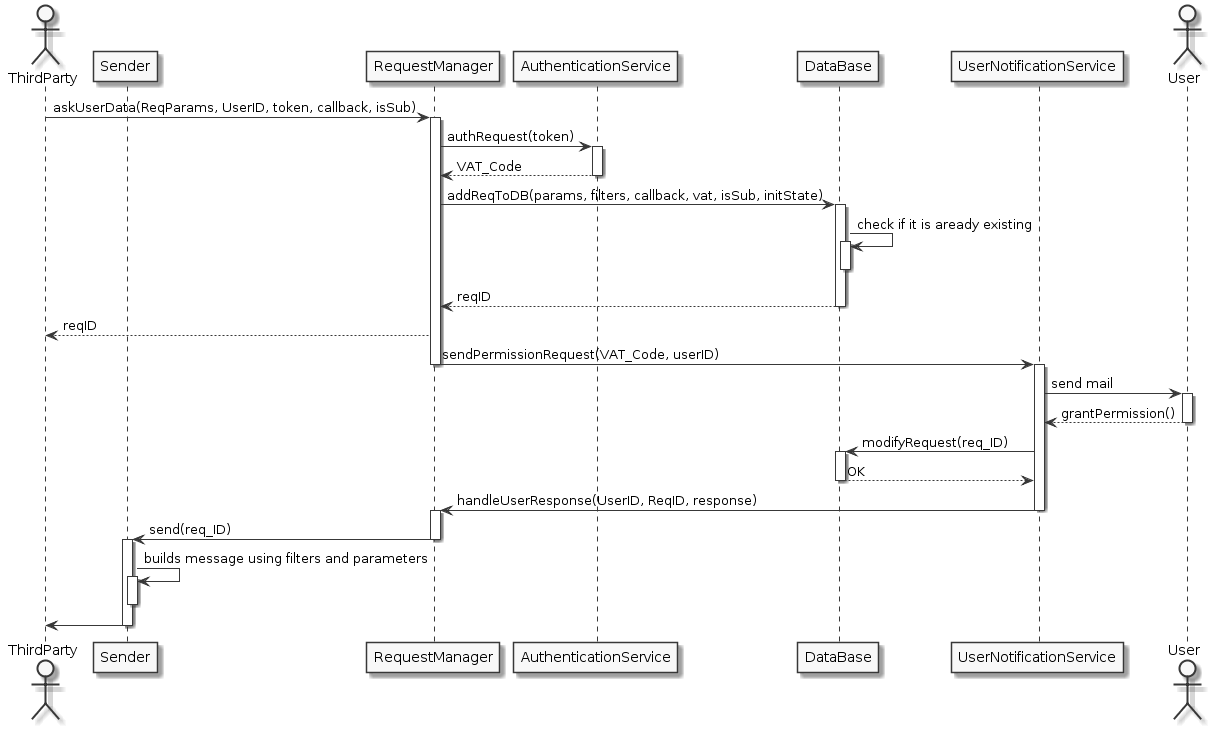
\includegraphics[width=\columnwidth]{singleuser_seq.png}
	\caption{Single User Data Request Sequence Diagram}
\end{figure}
\FloatBarrier

\subsubsection{Group Data Request}
In case of group data requests, no user authorization is needed.
The only thing that must be checked is if the number of users in the target group is high enough to protect users' privacy. This task is carried out by a dedicated service which is invoked synchronously.
The corresponding response shall be then sent to the third party who made the request.

\FloatBarrier
\begin{figure}[!h]
	\centering
	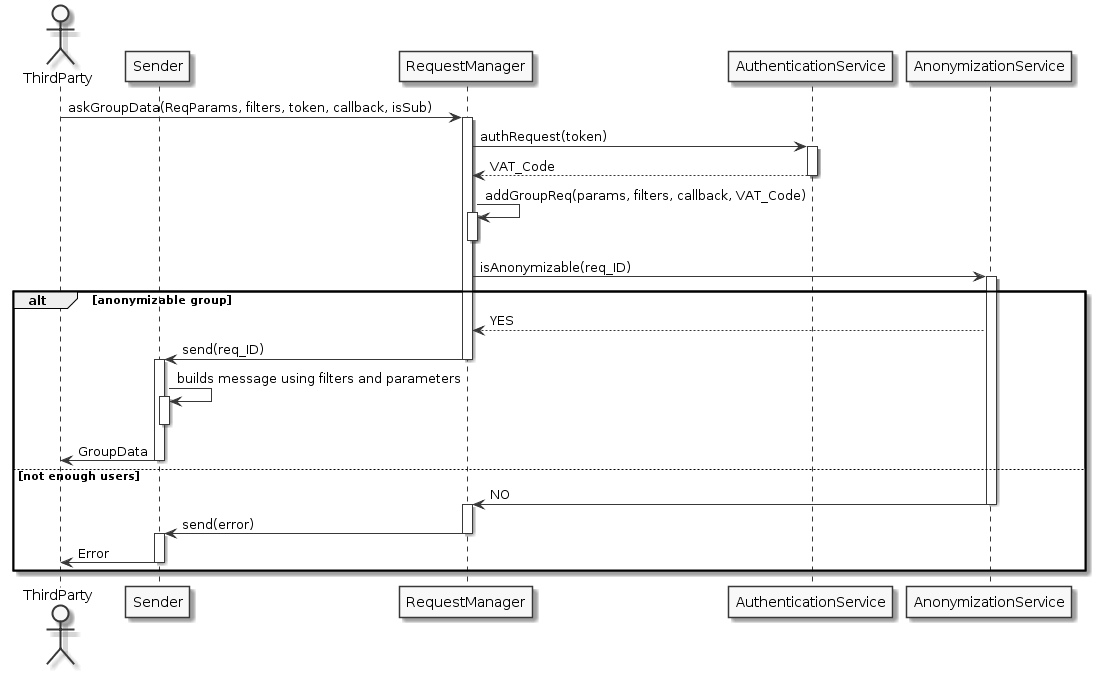
\includegraphics[width=\columnwidth]{group_seq.png}
	\caption{Group Data Request Sequence Diagram}
\end{figure}
\FloatBarrier

\subsection{Component Interfaces}
In the following diagram the main methods of the system's components are described in order to explain their interactions. These interfaces and methods are needed whatever the implementation of the underlying component will be, to guarantee that the whole system will meet its functionalities.
Asynchronous communication between components is represented with dashed lines and in the receiving components, the \textit{handleMessage()} function is called when a message is received.

\FloatBarrier
\begin{figure}[!h]
	\centering
	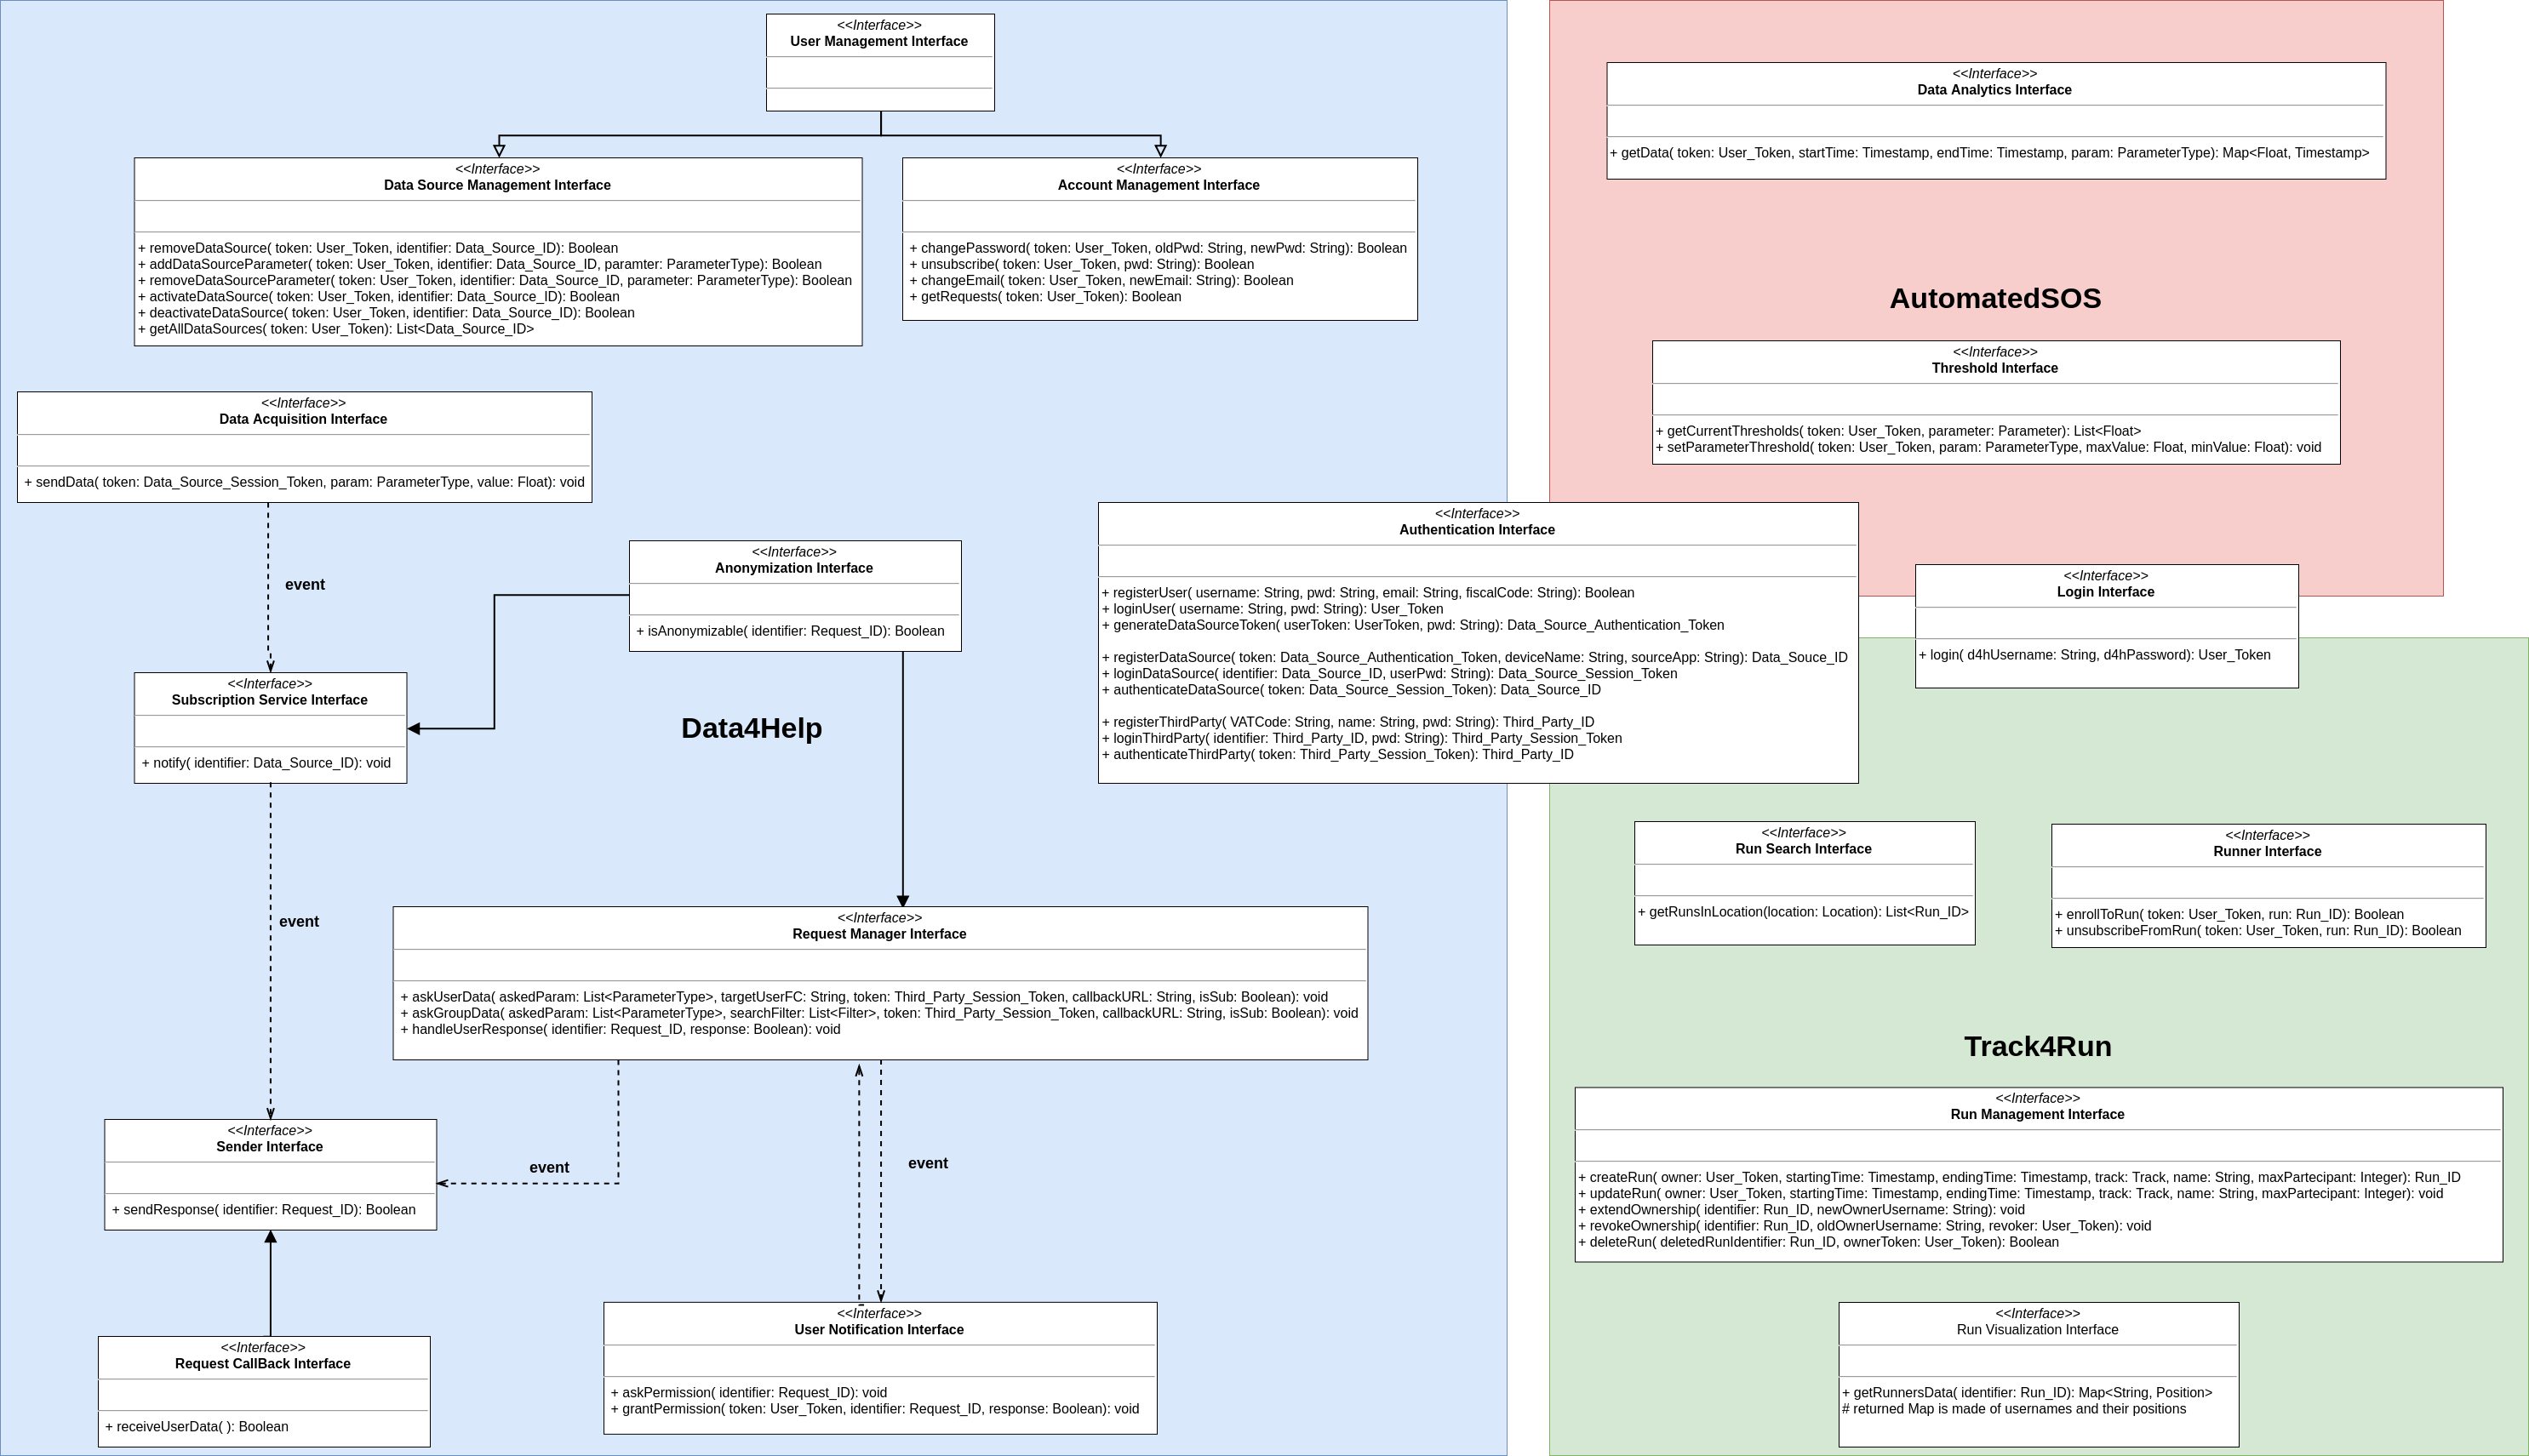
\includegraphics[width=\columnwidth]{ComponentInterfaceDiagram.png}
	\caption{Component Interface Diagram}
\end{figure}
\FloatBarrier

\subsection{Selected Architectural Styles and Patterns}

\begin{itemize}
	\item \textbf{Loose Coupling}: the first principle we followed in the design of the whole product is loose coupling, which means that we tried to minimize the dependencies between components of a subsystem and between the three subsystems as well. This means that each subsystem can be developed, deployed and maintained separately, which gives to the system a good flexibility for future development.
	\item \textbf{Stateless Components}: since one of our major concerns is the reliability of our system and how it recovers from failures, our components are designed to be stateless. This means that each component reads and writes on a DB at every step of its work, so that if one of the services is temporarily down, its state can be easily recovered from the DB.
	\item \textbf{Microservice Architecture Pattern}: For Data4Help we decided to implement a microservice architecture pattern. The idea behind a microservice-based architecture is to apply the \textit{SOA} (\textit{Service Oriented Architecture}) pattern  inside a big project by breaking it down in smaller pieces that act independently, communicate asynchronously and can be deployed in any fashion and number. This pattern is used in Data4Help because the achievement of high availability and scalability can be easily reached by decoupling the single functions of the system and deploying them independently in large numbers.
	
	In particular, for this microservice design we decided to adopt the following principles:
	
	\begin{itemize}
		\item \textbf{API Gateway Pattern}: A single entry point is provided for external access to the services. This gateway will then redirect the incoming calls to the single services. This gives us the possibility to keep together the request authentication management, load balancing and eventually performance testing. Notice that also the gateway can be scaled by adding another one with the same service registry in common.
		\item \textbf{Server Side Discovery}: This method is a way of keeping track of which are the services available on the system and where their instances can be found. It uses a \textit{Service Registry} at a known location where new services register themselves when deployed, so that the Gateway/Load Balancer can read the register to know where to redirect requests.
		\item \textbf{Asynchronous Queuing}: This pattern is used together with the \textit{Event Driven Architecture} pattern to achieve asynchronous and non-blocking communication between services. In our case, we implement asynchronous queuing when using message queues for sharing information and notifications between services. In this way, when a service A calls a service B, it only has to send a message and then it can continue with his job, even if the other service is temporarily unavailable.
		\item \textbf{Access Tokens}: In order to access any service of the system, external requests must include an access token. This token is used to identify and authenticate the actor who is performing the request.
	\end{itemize}

	\item \textbf{REST}: When asynchronous communication is not possible or desirable, for example during external calls to the system's services, a REST architecture is used to build RESTful APIs that can be accessed by software written in any language. This is another way in which we decouple the functions of our system.
	\item \textbf{MVC}: For AutomatedSOS and Track4Run subsystems, we decided to adopt a standard \textit{Model-View-Controller} monolithic architecture. This gives the possibility to the developers of this subsystems to use well-known commercial solutions to implement these applications.
	\item \textbf{Client-Server Pattern}: The classical separation of the MVC pattern between Model and View is strengthen using the client-server pattern, where there is a client asking for a resource and a server that must provide it. For AutomatedSOS and Track4Run the client is a \textit{thick-client} which takes care of the whole presentation part, whereas in the Data4Help subsystem we have a \textit{thin-client} application for the users, which sits on their browser.
\end{itemize}

\subsection{Other Design Decisions}
Some implementation-level solutions have been explored to better understand the problems that could occur during the implementation phase.

In particular, these are some technologies that have been taken into account:

\begin{itemize}
	\item \textbf{NoSQL Databases}: One of the key features of these kind of databases is scalability, and apparently they are very well integrated in many frameworks used for developing microservices. For this reason these kind of databases should be taken into account.
	\item \textbf{JWT}: JSON Web Tokens are a web authentication standard. They are lightweight, cross-platform, encrypted and easy to use. Alternatively, a possible solution for the authentication could be using \textit{OAuth2} servers.
	\item \textbf{Containers}: containers are used a lot in microservices deployment, and should be considered for the implementation of the Data4Help subsystem: they have some security drawbacks with respect to virtual machines or other cloud-based solutions. On the other hand, they are a fast and reliable way to manage many instances in a microservice cluster.
	\item \textbf{Proactive Monitoring}: tools like \textit{Prometheus} enable metric analysis and monitoring inside a microservice cluster. These tools can be easily used to identify a lack of computational power and dynamically scale our application.
\end{itemize}